\documentclass[12pt]{article}

% pacotes
\usepackage{sbc-template}
\usepackage{graphicx,url}
\usepackage{orcidlink}
\usepackage[utf8]{inputenc}
\usepackage{amsmath}
\usepackage{float} % para usar [H] nas figuras

\sloppy

% HEADER
\title{Comparativos de Algoritmos de Ordenação\\Análise de Complexidade}

\author{Izabel Oliveira da Paz Chaves\,\orcidlink{0009-0008-9198-3909}}

\address{Instituto de Ciências Exatas e Informática -- Pontifícia Universidade Católica de Minas Gerais \\ (PUC - Minas)\\ Caixa Postal 30535-610 -- Belo Horizonte -- MG -- Brazil\\ E-mail: \email{iopchaves@sga.pucminas.br} \\ ORCID iD: https://orcid.org/0009-0008-9198-3909 }

\begin{document} 

\maketitle

\begin{abstract}
  This article consists of a performance analysis of classical sorting algorithms, consisting of comparing the execution times, the number of comparisons and the number of movements performed by the following algorithms: Selection Sort, Insertion Sort, Bubble Sort and Quicksort.
\end{abstract}
     
\begin{resumo} 
  Este artigo consiste em fazer uma análise de desempenho dos algoritmos clássicos de ordenação, consistindo em comparar os tempos de execução, os números de comparações e o número de movimentações realizadas pelos seguintes algoritmos: Ordenação por Seleção (Selection Sort), Ordenação por Inserção (Insertion Sort), Ordenação por Bolha (Bubble Sort) e Quicksort.
\end{resumo}

\section{Informações Gerais}

Para o teste foram gerados quatro vetores diferentes com 100, 1.000, 10.000 e 100.000 elementos aleatórios a serem ordenados, contando os tempos de execução (em milissegundos), os números de comparações e os números de movimentações realizadas para os principais algoritmos de ordenação.

Foi utilizado o editor de texto Vim em um ambiente de nuvem da Google Cloud Console via linha de comando (CLI), sem interface gráfica. A linguagem de programação Java foi escolhida para fazer o comparativo entre as ordenações, enquanto a linguagem Python com as bibliotecas Pandas e Matplotlib foram utilizadas para gerar os respectivos gráficos.

\subsection{Ambiente de Execução}

Os testes foram realizados com o seguinte ambiente de software:

\begin{itemize}
  \item \textbf{Sistema}: Google Cloud Shell (CLI)
  \item \textbf{Google Cloud SDK}: versão 518.0.0
  \item \textbf{Editor de texto}: Vim 9.1 (compilado em 01 de abril de 2025)
  \item \textbf{Java}:
  \begin{itemize}
    \item OpenJDK versão 17.0.14 (lançada em 21 de janeiro de 2025)
    \item OpenJDK Runtime Environment (build 17.0.14+7-Ubuntu-124.04)
    \item OpenJDK 64-Bit Server VM (build 17.0.14+7-Ubuntu-124.04, modo misto)
  \end{itemize}
  \item \textbf{Python}: versão 3.12.3
  \item \textbf{Pandas}: versão 2.2.3
  \item \textbf{Matplotlib}: versão 3.10.1
\end{itemize}

\section{Introdução} \label{sec:firstpage}

Dentre os algoritmos de ordenação, o mais estudado em termos de eficiência na complexidade temporal é o Quicksort, cuja maioria dos casos apresenta complexidade de $O(n \log n)$. A sua natureza de Divisão e Conquista quebra o problema em partes menores, resolvendo cada uma delas de forma independente e posteriormente combinando as soluções. Devido à recursão, seu comportamento é descrito por uma equação de recorrência, provada logicamente pelo Teorema Mestre (Cormen, Leiserson, Rivest e Stein, 2001).

A análise média para o número de comparações é dada por:

\[
C(n) \sim 1{,}386n \log n - 0{,}846n \quad \text{(Sedgewick e Flajolet, 1996, p.17)}
\]

Entretanto, não existe um algoritmo de ordenação ótimo para todos os casos, pois a escolha depende de fatores como quantidade de memória disponível e grau de ordenação inicial do vetor. Dessa forma, analisaremos não apenas o tempo de execução, mas também o número de comparações e de movimentações.

A Ordenação por Seleção, por exemplo, realiza poucas movimentações, mas percorre o vetor $n$ vezes para encontrar o menor elemento a cada passo. Já a Ordenação por Inserção tende a ser desfavorável em movimentações. Embora ambos sejam algoritmos de complexidade quadrática $O(n^2)$, o Bubble Sort apresenta piores desempenhos ainda, trocando elementos de forma ineficiente e gerando muitos casos desfavoráveis.

\section{Condução de Teste}

Os algoritmos de ordenação foram executados sobre vetores de tamanhos 100, 1.000, 10.000 e 100.000, preenchidos com números aleatórios. Para cada execução, foram registrados o tempo de execução (em milissegundos), o número de comparações realizadas e o número de movimentações necessárias para ordenar o vetor.

\subsection{Comparativos de Ordenação por tamanho dos vetores}

\begin{table}[H]
\centering
\caption{Resultados para Bubble Sort}
\begin{tabular}{|c|c|c|c|}
\hline
Tamanho & Tempo (ms) & Comparações & Movimentações \\
\hline
100 & 0 & 4.950 & 7.386 \\
1.000 & 9 & 499.500 & 695.706 \\
10.000 & 112 & 49.995.000 & 72.773.430 \\
100.000 & 13.964 & 4.999.950.000 & 7.196.866.866 \\
\hline
\end{tabular}
\end{table}

\begin{table}[H]
\centering
\caption{Resultados para Insertion Sort}
\begin{tabular}{|c|c|c|c|}
\hline
Tamanho & Tempo (ms) & Comparações & Movimentações \\
\hline
100 & 0 & 2.264 & 2.367 \\
1.000 & 3 & 232.844 & 233.848 \\
10.000 & 27 & 23.825.944 & 23.835.951 \\
100.000 & 2.587 & 2.403.380.776 & 2.403.480.784 \\
\hline
\end{tabular}
\end{table}

\begin{table}[H]
\centering
\caption{Resultados para Selection Sort}
\begin{tabular}{|c|c|c|c|}
\hline
Tamanho & Tempo (ms) & Comparações & Movimentações \\
\hline
100 & 0 & 4.950 & 276 \\
1.000 & 3 & 499.500 & 2.976 \\
10.000 & 149 & 49.995.000 & 29.994 \\
100.000 & 4.086 & 4.999.950.000 & 299.964 \\
\hline
\end{tabular}
\end{table}

\begin{table}[H]
\centering
\caption{Resultados para Quicksort}
\begin{tabular}{|c|c|c|c|}
\hline
Tamanho & Tempo (ms) & Comparações & Movimentações \\
\hline
100 & 0 & 616 & 849 \\
1.000 & 0 & 10.310 & 10.719 \\
10.000 & 1 & 139.567 & 130.848 \\
100.000 & 12 & 1.883.482 & 1.528.146 \\
\hline
\end{tabular}
\end{table}
É observada uma diferença nítida entre os tempos de execução dos algoritmos a partir de $10^4$ elementos, com melhor eficiência para o Quicksort. Em analogia ao Bubble Sort, o Selection Sort é mais rápido a partir de $10^4$ elementos. No entanto, ao considerar o número de movimentações realizadas, verifica-se que:

\[
\text{Movimentações do Bubble} \approx 26^n \times \text{Movimentações do Selection}
\]

onde a razão entre as grandezas foi estimada com base nos resultados obtidos. O número de comparações, contudo, permanece praticamente o mesmo para ambos os algoritmos.

O algoritmo de Insertion Sort, por sua vez, apresenta aproximadamente a metade do número de comparações do Selection Sort, enquanto o número de movimentações segue a relação:

\[
\text{Movimentações do Insertion} \approx 8{,}57^n \times \text{Movimentações do Selection}
\]

Essas deduções foram feitas por proporcionalidade entre os resultados observados para diferentes algoritmos de ordenação. Quanto maior a precisão e a acurácia dos números utilizados (considerando mais casas decimais), mais fiel será a aproximação em relação ao comportamento simulado.

Cabe destacar que o expoente $n$ utilizado nas relações é apenas uma representação da tendência quadrática dos custos, e não implica em um crescimento exponencial. Caso o comportamento fosse, de fato, exponencial, a proporcionalidade deveria ser expressa por $n \times n$ e não apenas $n$.

Por fim, observa-se no Quicksort a característica de crescimento assintótico relacionado à função logarítmica, condizente com sua complexidade média de $O(n \log n)$.

\section{Gráficos}

A seguir são apresentados os gráficos gerados em Python, utilizando Pandas e Matplotlib, a partir dos dados obtidos:

\begin{figure}[H]
\centering
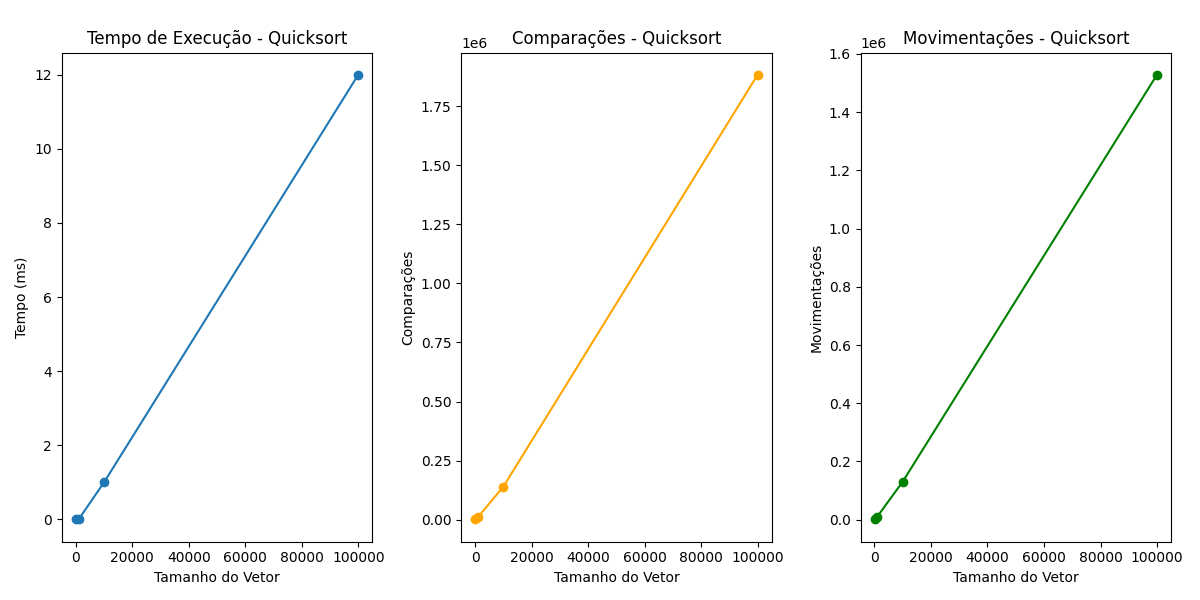
\includegraphics[width=0.7\textwidth]{grafico_quicksort.png}
\caption{Tempo de execução, Comparações e Movimentações no Quicksort}
\end{figure}

\begin{figure}[H]
\centering
\includegraphics[width=0.7\textwidth]{grafico_selecao.png}
\caption{Tempo de execução na Ordenação por Seleção}
\end{figure}

\begin{figure}[H]
\centering
\includegraphics[width=0.7\textwidth]{grafico_insercao.png}
\caption{Número de comparações no Algoritmo de Inserção}
\end{figure}

\begin{figure}[H]
\centering
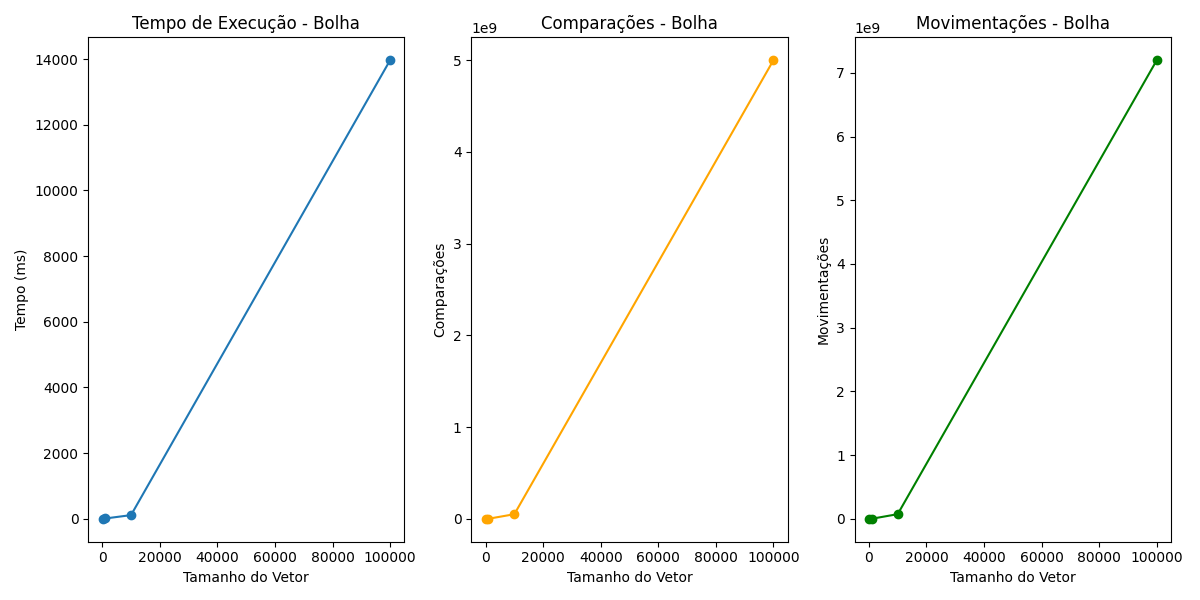
\includegraphics[width=0.7\textwidth]{grafico_bolha.png}
\caption{Tempo de Execução, Comparações e Movimentações no Bolha}
\end{figure}

% força fim dos gráficos antes das referências
\clearpage

\section{Referências}

\begin{thebibliography}{99}

\bibitem{cormen} Cormen, T. H.; Leiserson, C. E.; Rivest, R. L.; Stein, C. (2001). \textit{Introduction to Algorithms}. MIT Press.

\bibitem{sedgewick} Sedgewick, R.; Flajolet, P. (1996). \textit{An Introduction to the Analysis of Algorithms}. Addison-Wesley.

\bibitem{ziviani} Ziviani, Nivio (2013). \textit{Projeto de Algoritmos: com implementações em Java e C++}. 3ª reimpressão da 1ª edição de 2007. ISBN 978-85-221-0525-0.

\bibitem{knuth} Knuth, Donald E. (1997). \textit{The Art of Computer Programming, Volume 1: Fundamental Algorithms}. Addison-Wesley.

\end{thebibliography}

\end{document}
